\chapter{Related Work}
\label{chap:rel}

\minitoc

\vfill

Association rules mining is widely covered by existing work.
Before presenting our datasets of interest and
detailing why state-of-the-art solutions are not sufficient for such data,
we start by reviewing in this chapter related algorithms and methods.
As association rules are generated from itemsets,
this chapter mostly covers itemset mining.

Our core heritage from existing work are
notions and models for itemset and association rules mining.
These are presented in Section~\ref{sec:model} along LCM,
our algorithm of choice for closed itemsets enumeration.
We review more completely algorithms for itemsets mining in Section~\ref{sec:rel:fim}.
Some literature proposes to mine itemsets in parallel,
in order to speed up the computation or to tackle larger datasets.
This precisely echoes our needs, hence we discuss these propositions in Section~\ref{sec:rel:par}.

Most of this work focuses on frequent itemsets,
yet frequency is not always a good indicator of interest.
Therefore we also discuss, in Section~\ref{sec:rel:selection},
which quality measure can provide alternatives
and how they can be integrated in the analytics process.
Reviewing existing algorithms also shows the importance of the underlying structures and their implementation.
In practice, however, fast implementations are not published or difficult to re-use.
We illustrate this in Section~\ref{sec:rel:implems},
and show that our concerns on this topic led us to maintain \jlcm, our implementation of LCM,
as an open-source project.
The following chapters re-use \jlcm itself, or some of its components.

We conclude in Section~\ref{sec:rel:conclusion} by distinguishing
what we can borrow to existing work and what should be improved.


\pagebreak


\section{Mining itemsets and association rules}
\label{sec:model}

We will see in the next chapter that receipt records can be transformed in various ways,
depending on the desired associations' semantics.
Though, in all cases data has to fit a common model to be processed by our itemset mining algorithms.
We use Agrawal's model for association rules mining in transactional databases~\cite{AgrawalVLDB94},
with the restriction to closed itemsets~\cite{PasquierICDT99}.

In this section we start by defining this model and notions,
which will be used through the rest of the manuscript.
Then we focus on LCM, an efficient and parallelizable closed frequent itemsets mining algorithm~\cite{UnoDS04}.
%We finally present our implementation, \jlcm, and validate its performance.
\capa uses LCM at the mining step, and \toppi inherited from LCM its basic enumeration principles.
%We present and discuss other algorithms for itemset mining in Section~\ref{sec:rel:fim}.



\subsection{A model for itemset and association rules mining}
\label{sec:model:mining}

Mining itemsets requires the definition of a ground set of items, {\mf I}.
A {\em transaction}, usually denoted $T$, is a subset of {\mf I}.
Our mining algorithms' input is a transactional dataset {\mf D}, {\em i.e.} a collection of transactions.
An {\em itemset}, denoted $I$, is also subset of {\mf I};
we introduce another term in order to distinguish the input and the output of mining algorithms.
In mining programs and itemsets collections, items are represented as integers,
as the example in Table~\ref{tab:db}.

Abstracting the notion of item allows us to apply the same algorithms on datasets carrying various semantics.
%The associated semantic only appear in the curation and exploration steps of our analytics pipeline.
For example, if items are products,
then transactions may represent the receipt given to the customer after his purchase,
like $\{\mathit{bread, butter, grated cheese, noodles, cola}\}$.
In this case frequent itemsets (defined below) represent sets of products that are frequently purchased together,
{\em e.g.} $\{\mathit{bread, butter}\}$.
In the following we will also consider a case where $\cal I$ is the union of
demographic attributes' values and product categories.
Then, each receipt record may be converted into a transaction,
like  $\{\mathit{ <35, Male, \text{Ile-de-France}, Paris, cola}\}$.
In that case itemsets of interest, for instance $\{\mathit{ <35, Sodas}\}$,
would represent how a customer segment is akin to buy products from one of our taxonomy's categories.

\begin{table}
		\centering
		\begin{tabular}{|r|l|l|}
  \hline
  TID   & Transaction \\ \hline
  $t_0$ & $\{0,1,2\}$       \\
  $t_1$ & $\{0,1,2\}$       \\
  $t_2$ & $\{0,1\}$         \\
  $t_3$ & $\{2,3\}$       \\
  $t_4$ & $\{0,3\}$       \\\hline
\end{tabular}

		\caption{
			\label{tab:db}
			An example input ${\cal D}$.
			Transaction identifiers (first column) are indexes necessary to the storage system.
			In this dataset, the itemset $\{1,2\}$ has a support equal to $2$
			and $\mathit{closure}(\{1,2\})=\{0,1,2\}$.
			The itemset $\{3\}$ is closed and has a support equal to $2$.
			The projected dataset ${\cal D}[\{3\}]$ contains transactions $t_3$ and $t_4$.
			}
\end{table}

Given an itemset $I$,
a transaction $t$ is an {\em occurrence} of $I$ if $I \subseteq t$.
The number of occurrences of an itemset in ${\cal D}$ is called its {\em support},
denoted $\mathit{support}_{\cal D}(I)$.
When it's clear from the context we may omit ${\cal D}$ and note the support as  $\mathit{support}(I)$.
An itemset $I$ is said to be {\em closed} if there exists no itemset $I'\supseteq I$
such that $\mathit{support}(I) = \mathit{support}(I')$.
The number of closed itemsets, further abbreviated as {\em CIS},
is less important than the number of itemsets.
%(depending on the dataset, closed itemsets can be orders of magnitude less numerous),
Though, CIS provide the same amount of information on ${\cal D}$~\cite{PasquierICDT99}.
For example,
if $\mathit{support}(\{2,5,8\}) = \mathit{support}(\{2,5\})$,
then the latter can be dismissed.
Several algorithms therefore extract closed itemsets only,
in order to improve performance and avoid redundant results~\cite{PeiSIGMOD00,UnoFIMI04}.

\begin{definition}[Closure]
	The greatest itemset $I' \supseteq I$ having the same support as $I$ is called the {\em closure} of $I$,
	further denoted as $\mathit{closure}(I)$.
\end{definition}

The {\em projected dataset} for an itemset $I$ on a dataset ${\cal D}$ is the collection of occurrences of $I$:
${\cal D}[I] = \langle T \in {\cal D} \mid I \subseteq T \rangle$.
To further reduce its size, we always remove all items of $I$, yielding the {\em reduced dataset}:
${\cal D}_I = \langle T \setminus I \mid T \in {\cal D} \wedge I \subseteq T \rangle$.
Note that $\mathit{support}_{\cal D}(I) = \mathit{support}_{{\cal D}[I]}(I) = |{\cal D}_{I}|$.
Table~\ref{tab:db} shows a dataset and some closure examples.

In this work, we will mine closed itemsets in transactional datasets.
That is, we will find all closed itemsets $I$ matching a given criteria in a dataset $\cal D$,
along with each $\mathit{support}_{\cal D}(I)$.
The motivation of this computation is the generation of association rules~\cite{AgrawalSIGMOD93}:

\begin{definition}[Association rule]
	An association rule is an implication of the form $A \rightarrow B$,
	where $A \subseteq \cal I$, $B \subseteq \cal I$ and $A \cap B = \emptyset$.
	$A$ is the rule's {\em antecedent} and $B$ its {\em consequent}.
\end{definition}

The computation of $\mathit{support}_{\cal D}(A)$ and $\mathit{support}_{\cal D}(A \cup B)$
gives to the analyst a quick intuition
of how the purchase of product(s) $A$ leads to the purchase of product(s) $B$,
for example.
In another dataset (\textit{LastFM}, presented in Section~\ref{sec:model:conc}),
a transaction is a set of artists listened to by a single user.
Then an association $\{a,b\}\rightarrow\{c,d\}$ represents how many
listeners of artists $a$ and $b$ are also listeners of $c$ and $d$.




\subsection{Enumerating frequent closed itemsets with LCM}
\label{sec:lcm}

Given a frequency threshold $\varepsilon$,
an itemset $I$ is said to be {\em frequent} in a transactions set ${\cal D}$ if
$\mathit{support}_{\cal D}(I) \geq \varepsilon$.
%Several algorithms aim at mining closed itemsets (CIS) present in a dataset (see Section~\ref{sec:rel:fim}),
%most commonly {\em frequent} closed itemsets.
In this manuscript, we generally use absolute values for our frequency threshold,
whereas most of the literature on frequent CIS mining uses relative thresholds.
Indeed, marketing analysts involved in the \datalyse project are used to
absolute measures of their customer base.
For example, they may state they are interested in trends involving at least \num{1000} customers.
Such number is much more intuitive to them than its equivalent relative threshold in our tickets dataset: \num{0.0003}\%.

Among existing frequent CIS mining algorithms, we firstly present LCMv2~\cite{UnoDS04},
awarded the best implementation of the second workshop on Frequent Itemset Mining Implementations~\cite{FIMI04}.
It was also shown by Négrevergne {\em et al.}
that LCM can be efficiently parallelized on multi-core machines~\cite{NegrevergneHPCS10}.
As we are counting transactions and items in millions and targeting a distributed platform,
this potential for parallelization was a strong motivation when choosing LCM as our initial itemset miner.

LCM is a backtracking algorithm relying on two fundamental properties:
the {\em closure extension}, that generates new closed itemsets from previously computed ones,
and the {\em first parent} that avoids redundant computation.
We define these principles below.

\begin{definition}
	An itemset $J \subseteq {\cal I}$ is a closure extension of a closed itemset
  $I \subseteq {\cal I}$ if $\exists e \notin I$,
	called an {\em extension item}, such that $J=\mathit{closure}(\{e\}\cup I)$.
\end{definition}

LCM enumerates CIS by recursively performing closure extensions, starting from the empty set.
%Thus pruning the solution space means avoiding one or many recursive calls.

In Table~\ref{tab:db} (p.\pageref{tab:db}), $\{0,1,2\}$ is a closure extension of both $\{0,1\}$ and $\{2\}$.
This example shows that a new itemset can be generated by two different closure extensions.
Uno {\em et al.}~\cite{UnoDS04} introduced two principles
which guarantee that each closed itemset is traversed only once in the exploration.
First, closure extensions are restricted to {\em prefix extensions}:
only items smaller than the previous extension are allowed.
Furthermore, we prune extensions that do not satisfy the {\em first-parent} criterion:
%(which is equivalent to LCM's prefix-preserving closure extension):

\begin{definition}
	\label{def:firstparent}
	Given a closed itemset $I$ and an item $e \notin I$,
	$\langle e, I \rangle$ is the first parent of
	$J=\mathit{closure}(\{e\}\cup I)$ iff. $\mathit{max}(J\setminus I)=e$.
\end{definition}

\begin{algorithm}%[tb]
%\begin{small}
	\caption{LCM}
	\label{alg:jlcm}
  	\KwData{dataset $D$, minimum support threshold $\varepsilon$}
  	\KwResult{Outputs all frequent closed itemsets in ${\cal D}$}
	\Begin{
            $\bot_{closed} \gets  \bigcap_{T \in {\cal D}}\ T$\\
            \textbf{output} $\bot_{closed}$\\
            \ForEach{$i \in {\cal I}  \mid  i \not \in \bot_{closed}$}{
	      $expand(\bot_{closed},i,{\cal D},\varepsilon)$\label{line:LCMstart}
            }
	}

	%\setcounter{AlgoLine}{0}
 	\SetKwProg{myproc}{Function}{}{}
	\myproc{$\mathit{expand(I,i,{\cal D}_I,\varepsilon)}$}{
		\KwData{Closed frequent itemset $I$, extension item $i$, reduced dataset $D_I$, minimum support threshold $\varepsilon$}
		\KwResult{Outputs all closed itemsets containing $\{i\}\cup I$}
		\Begin{
      \If(\tcp*[f]{Frequency test}){$\mathit{support}_{{\cal D}_I}(\{i\}) \geq \varepsilon$}{ \label{line:LCMfrqTest}
		      $I_{ext} \gets \bigcap_{T \in {\cal D}_I[\{i\}]}T$ \tcp*[f]{Closure computation}\\ \label{line:LCMitemsetClosure}
		      \If(\tcp*[f]{$1^{st}$ parent test}){$\mathit{maxItem(I_{ext})} = i$}{ \label{line:LCM1stparent}
                        $J \gets I \cup I_{ext}$\\ \label{line:LCMjoinPPext}
                        \textbf{output} $(J,\mathit{support}_{{\cal D}_I}(\{i\}))$\\ \label{line:LCMoutput}
                        $D_J = \{T \setminus J \;|\; T \in {\cal D}_I[\{i\}]\}$ \\ \label{line:LCMdatasetRed}
			\ForEach(\tcp*[f]{Augmentations}){$j \in {\cal I}\setminus J \mid j < i $}{\label{line:LCMaugmentations}
			  $\mathit{expand}(J,j,{\cal D}_J,\varepsilon)$    \label{line:LCMrecCall}
			}
		      }
                    }
		}
	}
%\end{small}
\end{algorithm}


Algorithm~\ref{alg:jlcm} summarizes the main function of LCM.
The extension enumeration order and the first parent test
shapes the closure extensions lattice as a tree.
This is illustrated in
Figure~\ref{fig:lcm}, which shows the itemsets tree for the dataset in Table~\ref{tab:db}.
$\langle 1, \{2\}\rangle$ is the first parent of $\{0,1,2\}$,
but $\langle 0, \{2\}\rangle$ is not.
Therefore the branch led by $\langle 0,\{2\}\rangle$ is pruned.

These enumeration principles also lead to the following property:
\begin{property}\label{prop:starters}
  By extending $I$ with $e$,
  LCM can only recursively generate itemsets $J$ such that $\mathit{max(J)}=e$.
\end{property}

This property allows us, for any CIS, to know where it will be outputted in the enumeration.
This is fundamental, both for the parallelization of the enumeration,
and to prune the CIS tree as in \toppi (see Chapter~\ref{chap:toppi}).


\begin{figure}
	\centering
	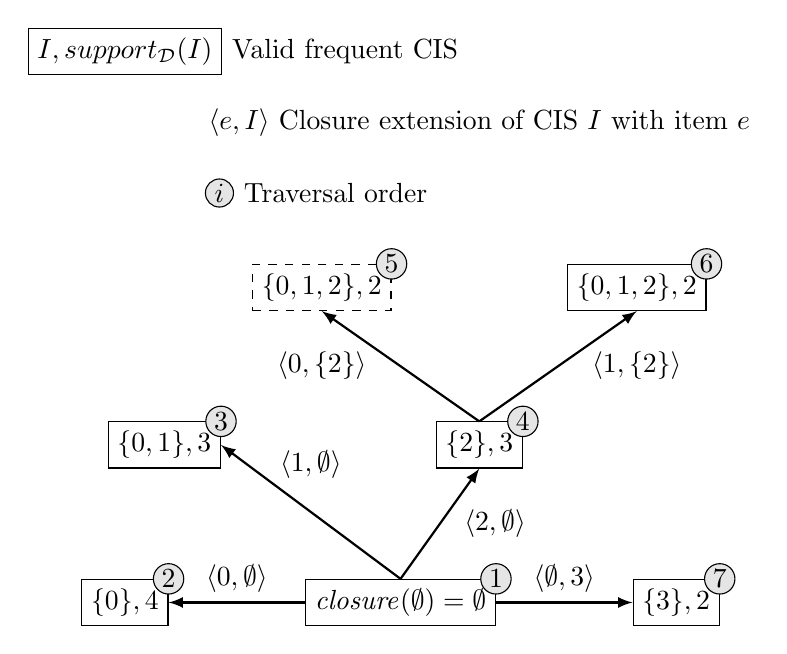
\begin{tikzpicture}[>=latex]
		\node (legenP)[draw,rectangle,minimum width = .8cm,minimum height=.5cm] at (-3.5,7) {$I,support_{\cal D}(I)$};
		\node [right] at (legenP.east) {Valid frequent CIS};

		\node (legenE) at (1, 6.1) {$\langle e,I\rangle$  Closure extension of CIS $I$ with item $e$};

		\node (legenC)[draw,circle,fill=gray!20,inner sep=1pt] at (-2.3,5.2) {$i$};
		\node [right] at (legenC.east) {Traversal order};

		\node (empty) [draw,rectangle,minimum width = .8cm,minimum height=.5cm] at (0,0) {$\mathit{closure}(\emptyset)=\emptyset$};
		\node (step0) [draw,circle,fill=gray!20,inner sep=1pt] at (empty.north east) {1};
		\node (0)     [draw,rectangle,minimum width = .8cm,minimum height=.5cm] at (-3.5,0) {$\{0\},4$};
		\node (step1) [draw,circle,fill=gray!20,inner sep=1pt] at (0.north east) {2};
		\node (1)     [draw,rectangle,minimum width = .8cm,minimum height=.5cm] at (-3,2) {$\{0,1\},3$};
		\node (step2) [draw,circle,fill=gray!20,inner sep=1pt] at (1.north east) {3};
		\node (2)     [draw,rectangle,minimum width = .8cm,minimum height=.5cm] at (1,2) {$\{2\},3$};
		\node (step3) [draw,circle,fill=gray!20,inner sep=1pt] at (2.north east) {4};
		\node (killed)[draw,rectangle,dashed,minimum width = .8cm,minimum height=.5cm] at (-1,4) {$\{0,1,2\},2$};
		\node (step4) [draw,circle,fill=gray!20,inner sep=1pt] at (killed.north east) {5};
		\node (012)   [draw,rectangle,minimum width = .8cm,minimum height=.5cm] at (3,4) {$\{0,1,2\},2	$};
		\node (step5) [draw,circle,fill=gray!20,inner sep=1pt] at (012.north east) {6};
		\node (3)     [draw,rectangle,minimum width = .8cm,minimum height=.5cm] at (3.5,0) {$\{3\},2$};
		\node (step6) [draw,circle,fill=gray!20,inner sep=1pt] at (3.north east) {7};
		\draw [->,thick] (empty.west) -- (0.east) node[above, midway] {$\langle 0, \emptyset\rangle$};
		\draw [->,thick] (empty.north) --(1.east) node[above, midway, yshift=0.3cm] {$\langle 1, \emptyset\rangle$};
		\draw [->,thick] (empty.north)--(2.south) node[above, midway, xshift=0.7cm, yshift=-0.3cm] {$\langle 2, \emptyset\rangle$};
		\draw [->,thick] (empty.east)--(3.west) node[above, midway] {$\langle\emptyset, 3\rangle$};
		\draw [->,thick] (2.north)--(killed.south) node[above, midway, xshift=-1cm, yshift=-0.3cm] {$\langle 0, \{2\}\rangle$};
		\draw [->,thick] (2.north)--(012.south) node[above, midway, xshift=1cm, yshift=-0.3cm] {$\langle 1, \{2\}\rangle$};
	\end{tikzpicture}
	\caption{\label{fig:lcm}
		Frequent CIS enumeration tree on our example dataset (Table~\ref{tab:db}), with $\varepsilon = 2$.
			$\langle e,I\rangle$ denotes the closure extension operation.
		}
\end{figure}


Figure~\ref{fig:lcm} also mentions in which order CIS are enumerated in LCM.
We now unroll this example enumeration:

\begin{enumerate}
	\item The algorithm starts by checking if any item in ${\cal D}$ appears in all transactions.
	Such items belong to the empty itemset's closure, $\mathit{closure(\emptyset)}$.
	As in most cases, here $\mathit{closure(\emptyset)}$ is empty.
	The empty set is therefore used as the initial itemset.
	It is extended by each frequent item in ${\cal D}$, called \textit{starter items}.

	\item The first starter is $0$, and $\{0\}$ is a closed itemset so the algorithm outputs it.
	As $0$ is the smallest item, no recursion happens.

	\item The next starter is 1, which generates by closure the itemset $\{0,1\}$.
	The closure satisfies the first parent test thus $\{0,1\}$ is outputted.
	The only remaining item in ${\cal D}_{\{0,1\}}$ is 2,
	but it's greater than the previous extension item so no recursion happens.

	\item The following starter is 2, leading to a closed singleton, $\{2\}$.
	Two frequent items, smaller than 2, remain in ${\cal D}_{\{2\}}$
	so the enumerator performs recursive extensions of $\{2\}$.

	\item The algorithm first extends $\{2\}$ with $0$ which, by closure, generates the pattern $\{0,1,2\}$.
	However, $\mathit{max}(\{0,1,2\}\setminus\{2\})=1>0$, so $\langle 0,\{2\}\rangle$ is not the first parent:
	this exploration branch is aborted.

	\item The next extension of $\{2\}$ is 1, which also closes to $\{0,1,2\}$.
	But this one satisfies the first-parent test so this CIS is outputted at this step.
	No further extension can happen because ${\cal D}_{\{0,1,2\}}$ only contains empty transactions.
	$\{2\}$ has no more extensions, so the algorithm backtracks to the starters.

	\item The last starter item is 3. $\{3\}$ is closed and valid,
	but no recursion happens because no frequent item remains in ${\cal D}_{\{3\}}$.
\end{enumerate}













\section{Itemset mining algorithms}
\label{sec:rel:fim}

LCM is not the first frequent CIS mining algorithm proposed in the literature;
we now review other itemsets mining algorithms
and discuss if they are relevant to mine large-scale datasets or retail data analysis.
We classify frequent itemsets mining algorithms into two families:
those defining frequency with a minimum support threshold, like LCM,
and those limiting the results set's size.
We start by presenting these two families.
We finally mention other definitions of the results set,
showing that these do not satisfy the requirements of marketing studies.



\subsection{Threshold-based frequent itemset mining algorithms}
\label{sec:rel:freq}

The first frequent itemset mining algorithm is APriori~\cite{AgrawalSIGMOD93,AgrawalVLDB94}.
Given a minimum frequency threshold $\varepsilon$ and a transactional dataset $\cal D$,
it computes all itemsets $I$ such that $\mathit{support}_{\cal D}(I) \geq \varepsilon$.

APriori introduced the generate-and-test approach,
which consists in iteratively generating a set of candidate itemsets,
then computing their support in the dataset.
The test phase of each iteration requires a pass on the complete dataset,
and candidates satisfying the frequency test are outputted progressively.
In its simplest variant,
APriori generates and tests itemsets of length $k$ during the $k$-th iteration.
The authors prove that the number of frequent itemsets decreases with their length $k$,
therefore APriori terminates when no more frequent itemsets are found.
This is a corollary of the {\em anti-monotony property},
also known as the {\em downward closure property}:

\begin{property}[Anti-monotony]
	\centering
	Given two itemsets $I$ and $J$,
	if $I \supset J$ then \\$\mathit{support}_{\cal D}(I) \leq  \mathit{support}_{\cal D}(J)$.
	\label{prop:antimonotony}
\end{property}

This property is leveraged by all frequent itemsets mining algorithms.
The generate-and-test approach is however less popular,
firstly because each test phase requires a complete scan of the dataset.
The second limitation is the number of candidates generated:
 in some cases most of them will not be frequent, and are therefore useless.
Both issues are particularly acute on our datasets,
where the number of items combinations can exhaust our machines' capacity,
and finding sequentially the support of many itemsets in gigabytes of transactions takes minutes, or even hours.

The first algorithm both reading the dataset once and enumerating only frequent itemsets is
Eclat~\cite{ZakiKDD97,ZakiTKDE00}.
Another algorithm having the same properties is FP-Growth~\cite{HanSIGMOD00,HanDMKD04},
who gained more popularity due to its internal representation of datasets.
Both algorithms avoid the generation of candidate itemsets by
traversing the itemsets lattice,
similarly to our example of Figure~\ref{fig:lcm}.
They also rely on succinct representations of the dataset,
which inspired the reduced datasets used in LCM and defined in Section~\ref{sec:model}.

FP-Growth starts by reading the dataset,
and stores all transactions in a prefix-tree.
Coupled with an indexing of items by decreasing frequency,
this results in a compact representation
because the prefixes containing very frequent items are merged in a few nodes of the tree.
FP-Growth then traverse the itemset lattice,
and generates a projected tree for each.
Prefix-trees are also efficient when used as itemsets indexes~\cite{LiuVLDB13}.

Pasquier et al. identified {\em closed} itemsets~\cite{PasquierICDT99},
which are typically one order of magnitude less numerous, while conveying the same information.
This definition paved the way for algorithms which, as LCM,
enumerate only closed itemsets to improve their efficiency.
The corresponding variants of FP-Growth are
CLOSET~\cite{PeiSIGMOD00} and its optimized version, CLOSET+~\cite{wangSIGKDD03}.

On our datasets, however, the instantiation of prefix trees is not amortized,
because between 90\% and 99\% of transactions are unique (we completely present our datasets in Section~\ref{sec:model:conc}).
This is close to prefix trees' worst case.
This phenomena worsens when the tree's nodes also store references to their supporting transactions,
as in the {\em Itemset-Tidset Search Tree}
at the heart of the CHARM algorithm~\cite{ZakiTR99,ZakiSDM2002}.

The inefficiency of prefix-trees over our datasets motivated our choice of LCM
as our initial CIS miner.
Its structures' efficiency is even more relevant in a multi-threaded setting,
as discussed in Section~\ref{sec:rel:multithreaded}.
We however do not implement the most complex variants of datasets in LCM,
namely the complete prefix tree of LCMv3~\cite{UnoOSDM05} and
zero-suppressed binary decision diagrams~\cite{MinatoPAKDD08}.
These are more relevant with dense datasets.

Overall this evolution of CIS mining algorithms shows the importance
of the underlying data structures, and their implementation.
For example, switching from node and pointers representations to array-based tries
can speedup FP-Growth by a factor of 10~\cite{RaczOSDM05}.



\subsection{Top-$k$ frequent itemset mining algorithms}

When confronted to a new dataset,
guessing a relevant minimum frequency threshold is not easy and usually requires a few attempts.
To overcome this usability problem,
some algorithms propose to instead ask the analyst how many itemsets she wants,
thus replacing the threshold $\varepsilon$ with a parameter $k$.
The algorithm then computes the $k$ most frequent itemsets in the dataset.
We refer to this approach as {\em global} top-$k$,
because a maximum of $k$ itemsets are mined for the whole dataset,
as opposed to the {\em per-item} top-$k$ itemsets we propose in Chapter~\ref{chap:toppi}.

Top-$k$ processing is a well studied research area in the domain of databases~\cite{IlyasACM08}.
A common case is the problem of top-$k$ query processing,
in which the goal is to identify the $k$ highest ranking items according to a query and a ranking function.
Efficient top-$k$ ranking algorithms are designed to identify the $k$ highest scoring results
without having to compute an exact score for every single item.
For instance, the TA algorithm~\cite{FaginPODS01}
compares the lowest score in the current version of the top-$k$
with an upper bound on the score of items that have not been processed yet.
The algorithm stops when it is sure that no more unseen item will have a score higher
than the $k$-th score so far.
It does so by comparing the dynamically maintained upper bound with the $k$-th score.
This early termination significantly reduces processing time while guaranteeing the same result
as when reading all solutions.
The two algorithms we present in this section,
and the \toppi algorithm presented in Chapter~\ref{chap:toppi},
rely on an analogous early termination strategy.

The computation of top-$k$-frequent itemsets was firstly solved by Han {\em et al.}
with the TFP algorithm~\cite{HanICDM02,WangTKDE05}.
Many of the most frequent itemsets in a dataset are actually singleton itemsets,
which are not revealing associations between items.
Hence TFP introduces another parameter, the minimum itemset length $l_{min}$.
Internally TFP relies on a frequent itemsets enumeration analogous to FP-Growth,
but TFP dynamically adjusts its frequency threshold depending on the support of the $k$ best current results.
Our preliminary experiments show that TFP is memory-consuming,
in particular when we release minimal length constraint, {\em i.e.} when $l_{min} = 0$.
Indeed, in this case the exploration strategy is almost greedy and TFP cannot prune prefix trees.

This was also observed by Chuang {\em et al.},
who proposed the MTK algorithm to circumvent this problem~\cite{ChuangVLDBJ07}.
MTK does not implement the minimum itemsets length constraint,
nor it relies on an FP-Growth-like enumeration of itemsets.
Instead MTK requires the user to define a memory usage limit
and uses a generate-and-test strategy.
The memory limit is converted into an upper bound on the number of candidate itemsets
to be generated and tested per database scan.
Because the number of candidates of length $i$ may not exhaust the memory capacity,
the authors also propose the $\delta$-stair search.
It consists in evaluating candidates of $\delta$ different lengths at each generate-and-test pass.
The $\delta$-stair search is more efficient in the MTK\_Close variant of the algorithm,
which mines the top-$k$-frequent CIS.
Indeed a non-closed itemset of length $i$ may have a closure of length $i+1$ or $i+2$.
As TFP, MTK finds during the exploration the minimum frequency ensuring the correctness of its results.

In Section~\ref{sec:toppi:xp:server} we need a global top-$k$ miner to build one of \toppi's baselines;
as the generate-and-test approach of MTK is inefficient on our datasets,
we instead implemented TFP with an additional optimization which compensates
our release of the minimal length constraint.



\subsection{Limitations of frequent CIS miners}

Although it is more convenient to define the output by its size rather than with a frequency threshold,
it does not change the order in which itemsets are considered by the algorithm.
Global top-$k$ algorithms are unable to compute frequent itemsets for rare items,
as this would require generating billions itemsets containing common items first.
In their experiments, the authors of the MTK algorithm set $k$ in $[100, 100000]$.
TFP is also tested on such large values of $k$, when $l_{min}=0$.
%Hence, similarly to our experiments with \jlcm in Section~\ref{sec:jlcm:validation},
%we observe that on our datasets of interest
Overall, whether they are using a threshold or top-$k$ approach,
frequent itemset mining algorithms return
results containing a negligible proportion of the available items.
Typically, results appearing less than \num{1000} or \num{10000} times are filtered out.
Hence frequent itemset mining hides the variety of large-scale datasets.

But frequency is not the only statistic able to characterize an itemset or an association rule.
We will see in Section~\ref{sec:rel:capa} that many quality measures have been proposed.
Although some of them can be integrated in an itemset mining algorithm,
on large-scale datasets this is prohibitive because it requires the enumeration of too many itemsets.
For the same reason, restricting the results set to itemsets that satisfy user-specified constraints,
as CAP~\cite{NgSIGMOD98}, is not feasible in our setting.


To overcome the overwhelming amount of results typically returned by itemset miners,
recent work defined highly-specialized classes of itemsets and proposed algorithms to mine them.
These classes of itemsets are often referred to as {\em concise representations}.
Closed itemsets were the first of such concise representations, and is lossless.
Surprisingly, this can be a downside: CIS are often too detailed for large-scale datasets.
Among the proposed classes we notice the {\em most informative} itemsets~\cite{Mampaey2011KDD,Mampaey2012TKDD} and the
{\em non-derivable itemsets}~\cite{calders2007non}.
Similarly, the KRIMP algorithm proposes to mine the itemsets that are the most efficient to compress the dataset~\cite{vreeken2011krimp}.

Overall these methods are not relevant in the retail domain,
because analysts may be interested in subtle variations of associations.
For example,
if {\em \{bread, butter, salt\}}, {\em \{bread, butter, salt, noodles\}} and {\em \{bread, butter, salt, rice\}}
have very similar supports,
then they might be considered as redundant by one of the previous approaches,
who will output at most one of them.
But their supports' similarity is itself an important information.
This motivated our focus on {\em frequent} itemset mining.
Although the vast majority of items are not covered by the results,
existing work provide efficient and reasonably complex routines and structures for frequent CIS enumeration.
We leverage these in the next chapters
in order to solve this detail-concision dilemma.
%This is further exposed in our experiments with \jlcm and \toppi.





\section{Parallel approaches}
\label{sec:rel:par}

Because of the important computation times incurred by itemset mining,
parallelization has been considered early on by the community.
We start by mentioning existing work on shared-memory systems,
which are similar to the sequential algorithms described previously.
Then we present distributed mining algorithms, focusing only on clusters of servers.
We do not review work on mining data distributed geographically,
across organizations or systems~\cite{KumarIIC06},
as it is not relevant in our application context.



\subsection{On shared-memory systems}
\label{sec:rel:multithreaded}

All algorithms relying on a traversal of the CIS space can assign distinct portions of this space to
different execution threads,
using properties analogous to our Property~\ref{prop:starters} (p.\pageref{prop:starters}).
Therefore most algorithms mentioned in Section~\ref{sec:rel:fim}
can leverage shared-memory systems to speed up the enumeration~\cite{ZakiDMKD97,LuccheseICDM07,ZaianeICDM01}.

Gothing {\em et al.} studied the memory accesses behavior and performance
of prefix-tree-based frequent itemset mining algorithms in ~\cite{GhotingVLDBJ07}.
Their experiments show the cache-inefficiency of these structures,
even though they use the fastest known public implementations at that time,
obtained thanks to the FIMI repository~\cite{FIMI03}.
For example they measure L3 hit rates below 40\%,
and less than 10\% of CPU utilization.
They overcome these bottlenecks by developing a
{\em tile-able cache-conscious prefix tree},
in which sub-trees are organized as tiles that fit in cache pages.
This is particularly compliant with cache pre-fetching strategies implemented by modern processors.
Their resulting implementation is up to five times faster,
and more importantly shows excellent speedups on multi-core and multi-processor systems.
The importance of cache-efficiency for multi-threaded itemset mining was also
identified by PLCM's authors~\cite{NegrevergneHPCS10}.

PLCM shows almost ideal speedups using simpler data structures
(transactions concatenated in an array).
These  are straightforward and CPU cache-friendly,
thus we used PLCM as a reference when implementing \jlcm, as shown in Section~\ref{sec:jlcm}.



\subsection{On clusters of servers or commodity machines}

The first distributed itemset mining algorithms follow APriori~\cite{CheungPDIS96,AgrawalTKDE96}.
Both distribute the generate-and-test approach
by distinguishing {\em local} candidates sets from
the {\em global} set of frequent itemsets ---
algorithms differ on whether candidates or transactions (or both) are exchanged across nodes.
As we discussed in Section~\ref{sec:rel:freq},
in our case the generate-and-test approach would hit the combinatorial explosion of itemsets.
This would be aggravated by shuffling candidate itemsets across the network.

At the time of writing
the MapReduce framework is widely available for distributed computing over commodity computers~\cite{DeanOSDI04}.
It has been popularized by the open-source implementation Hadoop~\cite{hadoop},
and the more recent Spark~\cite{ZahariaHC10}.
Both ensure reliably the distributed execution of user-defined functions,
and manage internally the data locality.
In MapReduce, data is considered as a collection of key-value pairs.
A {\em job} is the distributed execution of two functions: \verb|map| and \verb|reduce|.
At first,
\verb|map|:$(K,V)\rightarrow \langle K',V' \rangle$
is executed on each couple of the input data.
It can return an arbitrary number of couples,
which are not necessarily of the same type as the input's.
The system then groups the resulting couples by intermediate key.
For each distinct intermediate key (and its corresponding values), the system executes
\verb|reduce|:$(K', \langle V' \rangle) \rightarrow \langle K'',V'' \rangle$,
whose results are written to the job's output file.
The execution of \verb|reduce| is also distributed.
The execution system is coupled with a distributed storage,
hence the \verb|map| function is (ideally) executed locally,
on a machine storing a portion of the input couples.
This strategy allows a theoretically perfect parallelization of the \verb|map| execution,
and accounts for the important scalability of the framework.

The Spark framework provides a wider array of transformations of the dataset,
and does not constrain the programmer to a succession of \verb|map| and \verb|reduce| executions.
It can implement the MapReduce framework
but, as opposed to Hadoop, in Spark intermediate data is not necessarily written to disk.
Its extensive use of in-memory structures (particularly beneficial to iterative algorithms)
and a simpler, flexible API account for the recent popularity of Spark.
This however has a negligible impact on itemset mining programs,
who often need a fixed number of jobs.
Whether with Spark or Hadoop, the major time-consumers remain mining tasks,
therefore our distributed algorithms and experiments have not been migrated to Spark.

The academic and industrial success of these two systems
motivated the distribution of itemsets mining algorithms over the MapReduce framework.
Lin {\em et al.} developed a MapReduce implementation of Apriori~\cite{LinICUIMC12}.
Moens {\em et al.} also proposed two algorithms inspired by Eclat~\cite{MoensSML13}.
Although these parallel algorithms can handle large-scale datasets,
they inherit the initial drawback of frequent itemset mining:
most items do not appear in results.
For example, even items occurring \num{10000} times are usually filtered out in~\cite{MoensSML13}.

PFP, the first itemset mining algorithm proposed for MapReduce overcomes the problem of items coverage;
we now detail it more particularly because we use it as a baseline for \toppi's Hadoop version
(in Section~\ref{sec:toppi:xp:hadoop}, p.\pageref{sec:toppi:xp:hadoop}).



\subsection{PFP: Parallel FP-Growth}
\label{sec:rel:pfp}

Parallel FP-Growth~\cite{LiRecSys08} (PFP) proposes a slightly different computation:
for each frequent item in the dataset, PFP mines at most $k$ itemsets containing this item.
Their notion of frequent item is unusually large,
as they show examples supported by only 6 transactions out of 16 millions.
Thus PFP can provide itemsets covering the majority of the available items.

\begin{figure*}[tb]
	\centering
	\begin{scriptsize}
	\def\svgwidth{\linewidth}
	\input{svg/pfp.pdf_tex}
	\end{scriptsize}
	\caption{\label{fig:pfp}PFP's data flow}
\end{figure*}

Along the dataset $\cal D$, PFP has 3 parameters:
a minimum frequency threshold $\varepsilon$,
a maximum number of itemsets to return per item, $k$,
and a number of groups $\cal G$.
Each group corresponds to an independent mining task,
and these tasks are distributed in the cluster.
As depicted by Figure~\ref{fig:pfp},
the execution of PFP is divided in 3 MapReduce jobs.
%the two first jobs' input is $\cal D$,
%the last job reads the second job's output.
The complete algorithm unfolds as follows:

{
\renewcommand{\labelenumi}{Job \circled{\theenumi}}
\begin{enumerate}
	\leftskip .2in
	\item PFP counts the support of individual items in the dataset.
	Then it orders them by decreasing frequency,
	and assigns each one to a group in a round-robin fashion.
	Thus the most frequent item is assigned to group 1,
	the second most frequent to group 2,
	the ${\cal G}+1$ most frequent to group 1, etc.
	This ensures that the $\cal G$ most frequent items are dispatched to distinct groups,
	ensuring the balancing of the next job.

	\item In this job, group identifiers are used as intermediate keys.
	The \verb|map| function copies each transaction to each group its items belong to.
	Therefore the \verb|reduce| function processing an items group $g$ has enough transactions to mine
	all the itemsets containing items from $g$,
	and more particularly
	the frequent itemsets $I$ such that $\mathit{max}(I)$ belongs to $g$~\footnote{
	Because of this specification, PFP does not need to copy transactions entirely in the \verb|map| phase.
	See Section 2.4.1 in \cite{LiRecSys08}.
	}. As item groups are dispatched among workers,
	this ensures a distribution of the itemsets space in the cluster.
	Mining relies on FP-Growth~\cite{HanSIGMOD00}, presented in Section~\ref{sec:rel:freq},
	but each \verb|reduce| function only mines the $k$ most frequent itemsets in its group's transactions.

	\item Items are the intermediate key of this MapReduce job,
	which processes the results of the mining job.
	For each itemset $I$, the \verb|map| function outputs a couple $(i, I), \forall i \in I$.
	Thus each \verb|reduce| functions holds, for the given item $i$,
	all itemsets containing $i$ discovered by the previous job.
	Each execution of \verb|reduce| only outputs the $k$ most frequent itemsets,
	so the output file contains at most $k$ itemsets for each item $i$.
\end{enumerate}
}

PFP's mining phase has a single top-$k$ heap per group of items,
thus it generates at most $k$ itemsets per items group.
%PFP instantiates a separate heap per item only in its last job and fills them using the results of the mining phase.
It is therefore unlikely to obtain the required $k$ itemsets for an item with a low frequency because,
during the mining,
itemsets corresponding to more frequent items of its group will fill the heap.
PFP also does not ensure that itemsets found for each item are the most frequent, nor that they are closed.
We discuss in Section~\ref{sec:toppi:xp:hadoop}
how these factors impact the results for rare items,
and show experimentally that its coverage of items is sparser than expected.






\section{Selecting itemsets and association rules}
\label{sec:rel:selection}

So far we mostly mentioned frequent itemsets mining algorithms,
because these are efficient and
unveil prominent associations in datasets.
But this is not the case when a dataset contains more than a few thousands items.
Frequent itemsets usually combine frequent items with each others and,
because of the many possible combinations,
frequency is often not sufficient to distinguish surprising associations among the numerous frequent itemsets.
This is even more pronounced with a million items.

Two approaches can circumvent this problem:
we can either rank the discovered association rules
using a quality measure borrowed to statistics,
or we can restrict the itemsets mining according to such measure.
We now review how these two approaches have already been experimented in existing work.


\subsection{Rule ranking}
\label{sec:rel:capa}

In order to select less than a hundred association of particular interest,
and without additional knowledge like prices or users' ratings,
we can only evaluate an association $A \rightarrow B$ by comparing
$\mathit{support}(A)$, $\mathit{support}(B)$, $\mathit{support}(A \cup B)$
and the size of the dataset, $|\cal D|$.
This is proposed by extensive work in statistics and data mining,
as summarized in~\cite{GengACM06}.
In this survey, Geng \textit{et al.} review as many as 38 measures for association rules.
They also discuss 4 sets of properties like symmetry or monotony,
and how each of them highlights different meanings of ``rule quality'', such as novelty and generality.
But this still leaves too many choices for an analyst trying to find a ranking measure.


These 38 measures are also compared in~\cite{LeSANER15}.
Authors consider the case of extracting and ranking temporal rules ($\mathit{event\ A}\rightarrow\mathit{event\ B}$)
from the execution traces of Java programs.
Each measure is evaluated by its ability to rank highly rules known from a ground truth:
the Java library specification.
This experimental evaluation allow the authors to recommend one quality measure,
the {\em Odds Ratio}~\cite{McHughMB09},
as it is the best at highlighting associations expected according to the ground truth.
However we cannot state if this choice is also relevant on retail or Web data.

Another question raised by the number of quality measures available is:
do they rank really differently?
This is all the more relevant as most of them are designed
to filter according to a user-defined threshold (as frequent itemset miners do with $\varepsilon$).
This is observed by \textsc{Herbs}~\cite{Lenca2007,VaillantDS04},
which relies on a different and smaller set of measures than~\cite{LeSANER15}.
In their experiment, authors generate association rules,
rank them according to each measure,
and compare each pair of rankings using Kendall's $\tau$ correlation measure~\cite{KendallBIOMETRIKA38}.
They finally use these pairwise comparisons to cluster the ranking measures.
This clustering distinguishes 4 families of analogous rankings among the 20 measures tested.
One of these families contains almost a dozen measures which are very similar to ranking by {\em confidence};
{\em i.e.} $\mathit{support}(A \cup B) / \mathit{support(A)}$.
They also study the analytical properties of each measure,
and observe that measures belonging to the same experimental family often verify the same properties.
Though, \textsc{Herbs}' experiments rely on smaller datasets than ours.
The datasets used are from the health and astronomy domains,
and each of them contains at most \num{1728} transactions and leads to the extraction of 49 to \num{6312} rules.
As the size of the dataset has an impact on most of the quality measures,
it may also impact the similarity of their rankings.

Overall, existing work provides many quality measures for association rules,
but does not provide enough material to reliably choose one to rank large-scale retail data.
This motivated the development of \capa,
presented in Chapter~\ref{chap:capa}.


\subsection{Mining statistically significant itemsets}
\label{sec:rel:lamp}

Ranking a collection of association rules supposes, of course, to firstly mine these associations.
Those usually result from frequent itemset mining.
In order to avoid this costly computation,
existing literature proposes another approach:
guiding the itemsets space traversal according to a statistical quality measure.

Le Bras {\em et al.} define in~\cite{LeBrasDM10} the {\em General Universal Existential Upward Closure} (GUEUC)
which is analogous to the frequency's anti-monotony,
and also allows to prune the itemsets lattice.
Authors show that 13 quality measures out of the 32 they study verify this property,
and integrate these in a generate-and-test mining algorithm.
The candidate generation uses the GUEUC to limit the candidate itemsets to those
potentially satisfying the score limit defined by the user.
As discussed in Section~\ref{sec:rel:freq},
the generate-and-test approach is however not suitable to large-scale datasets.

In~\cite{LiuICDE11}, Liu \textit{et al.} propose to use the $p$-value
(via {\em Pearson's $\chi^2$ test}) to select statistically significant association rules.
A low $p$-value shows a correlation between a rule's antecedent and consequent (left and right terms).
Authors also propose an exploration framework
where rules are grouped by consequent, then
traversed by progressively adding items to the antecedent.
The framework provides hints to help the user to guess how each
additional item would make a difference.
On large-scale datasets,
this method raises resource issues
because the system should hold the whole dataset in memory during the exploration,
and each step may take too much time to meet the requirements of interactive applications.
This interactive process is also not suitable to our application case (presented in Chapter~\ref{chap:model}),
as the user would have too much choices among the available items.

Another integration of the $p$-value in the mining algorithm is proposed by LAMP~\cite{MinatoKDD14}.
It mines a transactional dataset $\cal D$
where each transaction is annotated positively or negatively.
In biology, this annotation may distinguish which persons in the dataset
suffer from a disease, for example.
Given a maximal $p$-value threshold $\alpha$,
LAMP will find all itemsets in $\cal D$ which are significantly correlated to positive annotations,
{\em i.e.} having a $p$-value smaller than $\alpha$ (using Fisher's exact test).
Minato {\em et al.} show that,
given the number of frequent itemsets according to a threshold,
we can compute a lower bound on the $p$-value of itemsets whose support is equal to the threshold.
This lower bound is increasing as the threshold decreases,
and may therefore exceed $\alpha$ for some value;
in this case we hit the greatest threshold guaranteeing that we are not missing any highly-correlated itemset.
This however requires to find the number of frequent itemsets in the dataset for each thresholds.
LAMP iteratively adjusts a threshold and mines the corresponding frequent CIS,
until the threshold converges to a value ensuring the results' correctness.


Both of these works aim at finding highly-correlated itemsets,
which requires the analyst to set a threshold on the $p$-value.
This is common practice in biology,
but less meaningful in the retail industry
where the challenge is instead on ranking association rules.
We also observe that these algorithms do not significantly
reduce the number of solutions traversed.
LAMP is even running LCM multiple times before producing its final results.
Thus we consider that closed itemsets should be firstly mined by frequency,
then ranked using a user-defined criteria.








\section{Implementations availability}
\label{sec:rel:implems}

So far we only discussed algorithms.
But we remark that the quality of their implementation has a strong impact on their performance.
As we experiment on unusually large transactional datasets,
in our case this performance is a condition of usability.
In this section we therefore discuss the issue of implementations availability,
starting with the case which raised our concerns, PFP.
We also present our LCM implementation, \jlcm,
and explain why we released it as an open-source library.


\subsection{The need for open source implementations}

PFP was firstly available in Mahout,
an open-source collection of machine learning algorithms for Hadoop~\cite{mahout}.
This implementation has not been maintained in the project,
and even deprecated in version 0.9.
Later on, it has been re-implemented from scratch in MLlib~\cite{mllib}.
This implementation does not match the algorithm described by Li {\em et al.}~\cite{LiRecSys08}
because it lacks a $k$ parameter\footnote{
Hence we stick to Mahout's implementation when comparing to PFP in Section~\ref{sec:toppi:xp:hadoop}.}.
MLlib thus implements a complete distributed frequent itemset miner,
which relies on an original, concise and elegant implementation of FP-Growth in Scala.
Our experiments suggest that this is not memory-efficient:
mining frequent itemsets from {\em LastFM}
using a frequency threshold of $0.01\%$
fails on our production cluster
(see specifications in Sections~\ref{sec:datalyse:prod} and \ref{sec:model:conc}, p.\pageref{sec:datalyse:prod}).
The same task (resulting in \num{7513} CIS) takes 20 seconds with \jlcm,
on the author's laptop with 2 threads and a Java heap of 1GB.
With MLlib's PFP mining tasks run out of memory,
or raise ``\verb|GC overhead limit exceeded|'' exceptions,
typically caused by algorithms instantiating too many small objects.
This is coherent with the observations on tree-based mining in~\cite{RaczOSDM05, GhotingVLDBJ07}.

%Albeit these performance issues, we should encorage such implementations.
Though, being part of a high-visibility project should allow the community to progressively enhance the implementation,
and provides baselines for further research, as ours.
Unfortunately such publication is not systematic (yet).
For example, for one of our experiments in Section~\ref{sec:toppi:xp:server}
we had to re-implement TFP~\cite{HanICDM02}.
We use the prefix-tree implementation from SPMF~\cite{FournierJMLR14},
another popular collection of mining algorithms.

Goethals and Zaki actively advocated for the publication of datasets and algorithms' source code,
by initiating two workshops on Frequent Itemset Mining Implementations~\cite{FIMI03,FIMI04}
and a workshop on Open Source Data Mining.
When concluding their report on the latter workshop,
Goethals {\em et al.} express their
``hope that the open source implementations of the presented algorithms may help many
researchers in the development of their own frequent pattern
mining algorithms and implementations.''~\cite{OSDM05}.

We share their need for re-usable and efficient building bricks for data mining.
Hence we released \jlcm, presented below, as a free software.
\jlcm is easily embeddable as a Java library via the Maven central repository.
Because of our regular use,
whether for preliminary experiments or in \capa,
we released 10 versions of \jlcm\footnote{\url{https://repo1.maven.org/maven2/fr/liglab/jlcm/jLCM/}}
including bug-fixing and feature releases.
\toppi will be released similarly upon its publication.



\subsection{\jlcm: our implementation of LCM}
\label{sec:jlcm}

We implemented LCM from scratch and in Java,
hence its name: \jlcm\footnote{\url{https://github.com/slide-lig/jlcm}}.
The choice of the Java language eases the Hadoop integration (in Chapter~\ref{chap:toppi}) and overall clarifies its API,
in particular when adding constraints to the exploration (as we do in Chapter~\ref{chap:capa}).
Thus \jlcm provides an important code base when implementing the following chapters' algorithms.
\jlcm is actually an implementation of the multi-threaded version presented by Négrevergne {\em et al.}, PLCM~\cite{NegrevergneHPCS10},
with two implementation optimizations adapted to large-scale datasets.

In PLCM,
invocations of $\mathit{expand}(\bot_{\mathit{closed}},i,{\cal D},\varepsilon)$
(Algorithm~\ref{alg:jlcm}, p.\pageref{alg:jlcm}, line \ref{line:LCMstart})
are dispatched to different threads for each item $i$.
Therefore each thread explores a different CIS branch:
Property~\ref{prop:starters} ensures that the threads' explorations are not overlapping.
Thus we can speed up the computation on large datasets, by using multi-core CPUs.

LCM was originally designed for mining smaller and denser datasets than ours, with high support thresholds.
Two internal operations (also performed by PLCM) have a completely different amortization on our sparse datasets.
These are the ``fast ppc'' (first parent test without closure computation) and ``anytime dataset reduction'',
performed by LCM at each step of the enumeration~\cite{UnoFIMI04}.
\jlcm does not always perform these operations.

Formally, the items set ${\cal I}$ is an ordered set of identifiers.
In practice, as \jlcm targets sparse datasets,
it uses a sparse representation of transactions
where a transaction of length $n$ only requires $n$ integers.
Our transactions representations leverage two additional optimizations.

\begin{itemize}
	\item The first one is Dynamic Element Reordering~\cite{ZakiSDM2002}.
	It is based on the intuition that, when we perform closure extensions with smaller items,
	it is more memory-efficient to index items from the most frequent to the least frequent,
	\textit{i.e.} 0 is the most frequent item.
	Indeed no smaller item exists so it will not lead to a recursive call,
	thus avoiding the construction of a huge projected dataset (line~\ref{line:LCMdatasetRed} in Algorithm~\ref{alg:jlcm}).
	Item indexes are updated (locally) in projected datasets,
	thus in $\mathit{expand(I,i,{\cal D}_I,\varepsilon)}$
	items smaller than $i$ have a greater support (in ${\cal D}_I$) than $i$,
	and greater items have a smaller support.
	This heuristic reduces the chances to fail the first-parent test.

	\item Another important optimization is a switch from Java's \verb|int| (32 bits)
	to \verb|short| integers (16 bits) when a projected dataset contains less than $2^{15}$ ($\num{32768}$) items.
	As LCM, \jlcm progressively reduces datasets by filtering out items which are no longer frequent.
	This is why recursive calls use the reduced dataset, ${\cal D}_I$ (Algorithm~\ref{alg:jlcm}, line~\ref{line:LCMdatasetRed}).
	Thus intermediate datasets tend to contain less and less items.
	Thanks to this phenomena the switch to \verb|short| integers is frequent.
\end{itemize}

Not only these techniques reduce the global memory consumption,
but because they reduce the size of the memory structures in deepest branches,
they also improve the CPU's cache hits.
This is important in a multi-threaded setting~\cite{NegrevergneHPCS10}.

The indexing by frequency however interferes with the ``natural'' items indexing
from the system in which our algorithms are integrated,
and imposes both a conversion of the input dataset and of resulting itemsets. % [ref to job 1 and 3 in \toppi].
For example, supermarket tickets refer to items with their International Article Number ({\em i.e.} bar code),
a 13 digit number requiring a \verb|long| integer (64 bits),
although most extracted datasets would need only a \verb|short|.
For a complete and streamlined integration of our work,
the transactions store should adopt \jlcm's indexation strategy,
or keep dataset views which are re-indexed by decreasing frequency.




\subsection{Experimental validation of our implementation}
\label{sec:jlcm:validation}

To assess the quality of our LCM implementation,
%as well as highlight the limitations of standard CIS mining,
we now compare \jlcm against the reference C++
implementation of PLCM~\cite{NegrevergneHPCS10}.
It is, to the best of our knowledge,
the current fastest parallel CIS mining algorithm.
This benchmark is done on a machine containing 4 Intel Xeon X7560 8-cores CPUs,
for a total of 32 cores.
This machine has a NUMA architecture: each CPU has a faster access to its closest 16GB memory block,
resulting in 64 GB of available RAM.

\begin{figure}
	\centering
	\begin{subfigure}[b]{0.48\textwidth}
		\includegraphics{fig/jlcm/allClosedRuntime/runtimePerSupport-lastfm.pdf}
		\caption{\emph{LastFM}}
		\label{fig:jlcmLastfm}
	\end{subfigure}
	\hfill
	\begin{subfigure}[b]{0.48\textwidth}
		\includegraphics{fig/jlcm/allClosedRuntime/runtimePerSupport-webdocs.pdf}
		\caption{\emph{WebDocs}}
		\label{fig:jlcmWebDocs}
	\end{subfigure}
	\caption{
		\jlcm and PLCM run-times w.r.t. frequency threshold $\varepsilon$.
	}
\end{figure}

Running times of both algorithms are displayed on
Figures~\ref{fig:jlcmLastfm} and~\ref{fig:jlcmWebDocs},
for \emph{LastFM} and \emph{WebDocs} (both presented in Section~\ref{sec:model:conc}).
Both algorithms are executed using 32 threads.
\jlcm's performance is comparable to PLCM for high thresholds ($\varepsilon$)
and \jlcm tends to be faster as $\varepsilon$ decreases.
For low values of $\varepsilon$, the dataset reduction can eliminate fewer items,
which means that the amount of memory transfers increases.
\jlcm has better memory management than PLCM, with more compact representations of datasets and NUMA awareness.
%\jlcm is able to detect when reduced datasets contain a low number of items
%and switches its internal representation to 16 bits per item identifier instead of the usual 32 bits.
This increases the benefits of the CPU cache and mitigates the problem of memory bandwidth.
Given that \jlcm was designed to operate at low support values, this result is encouraging.
Nevertheless, as $\varepsilon$ decreases,
the number of closed frequent itemsets increases exponentially, and so does the execution time.

This experiment validates our implementation:
\jlcm is comparable to PLCM in terms of run-time.
These results also show that traditional itemset mining approaches
are unable to generate itemsets for low support items in a reasonable amount of time.
With the lowest value of $\varepsilon$ used in this experiment,
the generated itemsets cover less than $1\%$ of the available items.
This phenomena, further discussed in Section~\ref{sec:model:conc},
does not only happen with Web data:
we also observe it with our retail datasets.













\section{Conclusion}
\label{sec:rel:conclusion}

In this thesis our main data representation is a transactional dataset,
usually denoted $\cal D$.
It is a collection of transactions, which are sets of items belonging to a ground set $\cal I$.
Many kinds of data can fit into this model:
a transaction can represent a supermarket ticket, an application user or a photo,
where items respectively represent products in a ticket, a user's favorite artists, or tags assigned to a photo.
We detail the different semantics of our datasets in the next chapter.


20 years of literature in the frequent itemsets mining field provides much details and experience
on efficient algorithms for itemsets enumeration.
Existing work also discusses the underlying datasets representations and algorithms implementations,
including on parallel systems.
Reviewing this literature led us to choose PLCM for preliminary experiments.
We re-implemented it in \jlcm,
released as an open source project %from the beginning of the present work
(the first release happened on February 2014).
As \jlcm is object-oriented, it provides us with useful and efficient building blocks
when implementing our contributions.
\jlcm also backs our first experiments,
showing that modern datasets
(counting both items and transactions in millions)
are not efficiently analyzed with existing itemset mining techniques.

The first problem is that existing algorithms cannot provide the analyst with an overview of the dataset,
that is itemsets about all items,
especially without requiring cryptic parameters.
To the best of our knowledge,
PFP is the itemset mining algorithm achieving the best coverage of items.
PFP is a MapReduce algorithm,
designed for large-scale datasets.
Our experiments, however, show that available implementations cannot mine our largest datasets.
As clusters of commodity computers relying on Hadoop are increasingly
the architecture of choice in academia and in industry,
we also consider to port our mining algorithm, \toppi, to this distributed platform.

Another problem is the selection of association rules.
Even when filtered by item (answering for example ``which sets of products are often associated with bread?''),
the associations are often too numerous,
or redundant when ranked by decreasing frequency.
Many quality measures have been proposed as alternatives to frequency,
but most measures are designed to filter associations having a score above a user-defined threshold.
Overall we cannot know from existing work how to rank interesting associations
in the retail domain, for example.

These two difficulties are respectively addressed by \toppi and \capa,
presented in Chapter~\ref{chap:toppi} and~\ref{chap:capa}.
Beforehand, Chapter~\ref{chap:model} describes the industrial setting in which \toppi and \capa are integrated.
